\chapter{Discovery of SARS-CoV-2 main protease inhibitors using a synthesis-directed de novo design model}\label{ch:ranking}

\begin{quote}
    This chapter is based on Aaron Morris, William McCorkindale, The COVID Moonshot Consortium, Nir Drayman, John D. Chodera, Savaş Tay, Nir London and Alpha A. Lee. Discovery of SARS-CoV-2 main protease inhibitors using a synthesis-directed de novo design model, \textit{Chem. Commun.}, 2021,57, 5909-5912 
\end{quote}

\noindent\hfil\rule{0.5\textwidth}{.4pt}\hfil

The SARS-CoV-2 main viral protease ($\mathrm{M}^\mathrm{pro}$) is an attractive target for antivirals given its distinctiveness from host proteases, essentiality in the viral life cycle and conservation across coronaviridae. We launched the COVID Moonshot initiative to rapidly develop patent-free antivirals with open science and open data. Here we report the use of machine learning for \emph{de novo} design, coupled with synthesis route prediction, in our campaign. We discover novel chemical scaffolds active in biochemical and live virus assays, synthesized with model generated routes.

Coronaviruses are a family of pathogens that is frequently associated with serious and highly infectious human diseases, from the common cold to the SARS-CoV pandemic (2003, 774 deaths, 11\% fatality rate), MERS-CoV pandemic (2012, 858 deaths, 34\% fatality rate) and most recently the COVID-19 pandemic (ongoing pandemic, 1.7 million deaths up to Dec 2020).

The main protease ($\mathrm{M}^\mathrm{pro}$) is one of the best characterized drug targets for direct-acting antivirals \cite{pillaiyar2016overview,cannalire2020targeting}. $\mathrm{M}^\mathrm{pro}$ is essential for viral replication and its binding site is distinct from known human proteases, thus inhibitors are unlikely to be toxic \cite{jin2020structure,liu2020development}. Moreover, the high degree of conservation across different coronaviruses renders $\mathrm{M}^\mathrm{pro}$ targeting a fruitful avenue towards pan-cornavirus antivirals \cite{ullrich2020sars}. To date, most reported $\mathrm{M}^\mathrm{pro}$ inhibitors are peptidomimetics, covalent, or both \cite{cannalire2020targeting}. Peptidomimetics are challenging to develop into oral therapeutics, and covalent inhibitors incur additional idiosyncratic toxicity risks. We launched the COVID Moonshot consortium in March 2020, aiming to find oral antivirals against COVID-19 in an open-science, patent-free manner \cite{chodera2020crowdsourcing}. 

Here we report the prospective use of a simple model to rapidly expand hits. Starting from 42 compounds with $\mathrm{IC}_{50}$ within assay dynamic range ($<100 \mu$M) and 515 inactives, our model designed 5 new compounds predicted to have higher activity, together with predicted synthetic routes. All designs were were chemically synthesized and experimentally tested, and 3 have measurable activity against $\mathrm{M}^\mathrm{pro}$. The top compound has comparable $\mathrm{M}^\mathrm{pro}$ inhibition to the best in the training set, but with a different scaffold, and is active against the OC43 coronavirus in a live virus assay. 

%Describe GenChem 
Algorithmic \emph{de novo} design aims to automatically generate compounds that are chemically diverse, synthetically accessible and biologically active \cite{schneider2016novo}. Classic approaches apply heuristics to fragment and modify known active compounds, with the region of chemical space explored and synthetic accessibility constrained by those rules \cite{brown2004graph,patel2009knowledge,hartenfeller2012dogs}. Recent machine learning approaches explore chemical space in more abstract molecular representation space \cite{gomez2018automatic,segler2018generating}, but this often comes at the expense of synthetic accessibility \cite{Gao2020Synthesizability}. Our approach builds on rule-based fragmentation and molecule generation, but employs a method that combines regression and classification amid noisy data, and use of machine learning to predict synthesis routes. Our model comprises two parts: compound prioritisation and chemical space exploration. 

%describe ranking model + result 
Our compound prioritisation model aims to predict whether a designed compound is likely to be an improvement in activity over the incumbent. However, as is typical in the hit-expansion stage, bioactivity modelling is hindered by insufficient data where the majority of compounds are inactive, and noisy data as measurement variability increases for lower affinity compounds. Thresholding the data and framing the problem as classification of active/inactive would not allow us to rank compounds based on predicted improvement over the incumbent, yet the amount of measured bioactivity data and the measurement noise makes a regression approach challenging.

% TODO - bigger discussion on QSAR modelling challenges


% TODO - include structure-based ranking PNAS paper? Proof of ranking-based approach.

To overcome both challenges, we develop a learning-to-rank framework \cite{duffy2010molecular,agarwal2010ranking}. Rather than training a regression model to predict the $\mathrm{IC}_{50}$ of a compound, we instead train a classifier to predict whether a compound is more or less active than another compound, with the input to the model being the \emph{difference} in molecular descriptors between the molecules (see Figure \ref{fig:roc_plot} for a schematic). This model accounts for both compounds with $\mathrm{IC}_{50}$ measurements and compounds that are simply inactive -- active compounds are ranked by their $\mathrm{IC}_{50}$, all inactives with no measurable $\mathrm{IC}_{50}$ are considered less active than active compounds, and inactive-inactive pairs are ignored. Further, we account for noise by only considering $\mathrm{IC}_{50}$ differences amongst actives above 5 $\mu M$. We use the FastAI Tabular model \cite{howard2018fastai}, with input features generated from concatenated Morgan, Atom Pair, and Topological Torsion fingerprints implemented in RDkit \cite{rdkit}, and dataset was randomly split into training (80\%) and testing (20\%); details about model implementation can be found in ESI and source code.

% TODO - include this section on elaborating on the ranking model
% Returning to the objective of this task, the goal is to find molecules that are more active, not merely classifying as active/inactive. Instead of formulating the task as a QSAR problem, an alternative line of attack is to consider pairwise ranking - given a pair of molecules $(A,B)$, is $A$ more active than $B$? This approach effectively combines `easy' classification and `difficult' regression into one `moderate' ranking task - binary classification of input pairs. In machine learning, this type of task is handled using models known as Siamese Neural Networks (SNNs) \cite{Koch2015SiamneseNN} where the the two inputs are encoded in the same way before their hidden states are operated on in unison to make a prediction. With a trained SNN, for scoring a drug candidate $X$ we can use the model prediction for $(X,Z)$ where $Z$ is the most potent active in the dataset.

% The SNN architecture that was used for this task also utilizes MPNNs (Fig \ref{fig:snn}). Both molecules from the input pair are passed through the same MPNN encoder to obtain their learnt graph embedding vectors; several fully-connected layers then operate on the vector difference between the graph embeddings to make the classification prediction. To enforce the antisymmetry of the model (so that $f(X,Y) = 1 - f(Y,X)$), all layer activations are tanh functions and the linear layers do not have any bias terms.
% \begin{figure}[!h] % !h ~ force here, t ~ top, b ~ bottom, p ~ separate page
% \centering
% 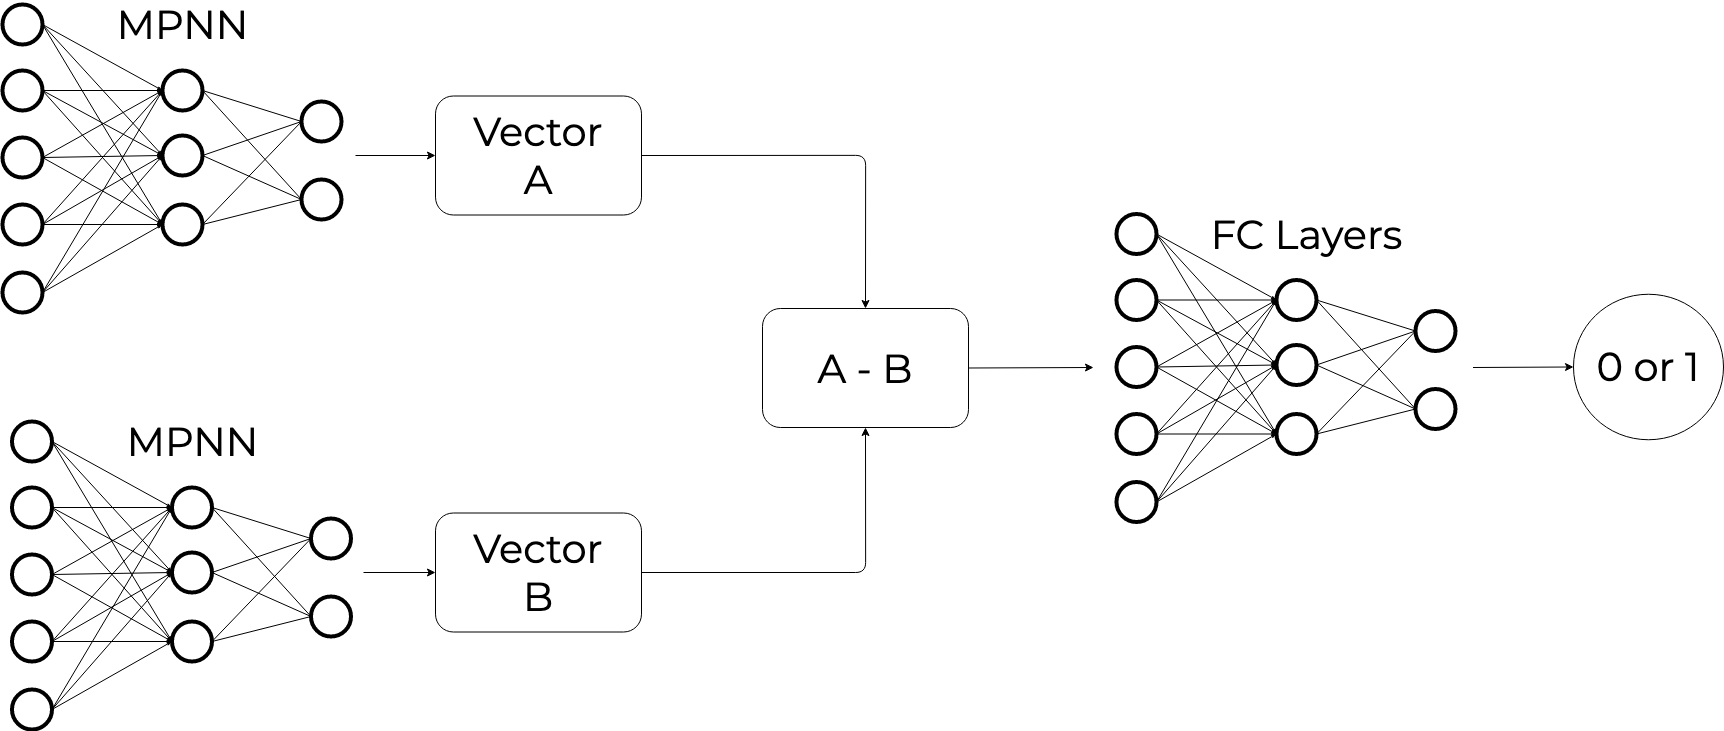
\includegraphics[width=\textwidth]{Chapter3/Figs/SNN.png}
% \caption{\label{fig:snn} An illustration of how the Siamese MPNN model is implemented.}
% \end{figure}

% To construct a suitable dataset for training the SNN, the activity data must be reformated into molecular pairs. This was done by pairing all actives with all inactives within each series, as well as pairing up actives where there is a significant activity difference ($\Delta$IC50 $>5\mu$M). The inactive molecules were not paired up between each other as the ranking of inactivity is not relevant to the task at hand and potentially noisy/misleading. The HTS data is also left out as the sheer size of that dataset leads to a computationally unfeasible number of molecular pairs even if the pairing is constrained by Tanimoto similarity. 

% A flipped pairing is included for all pairs so that the dataset is antisymmetric since the model would just predict ones otherwise. Theoretically this method is appealing because it is a natural way of oversampling the low proportion of actives, addressing the problem of dataset imbalance commonly seen in drug discovery classification tasks. Additionally, creating pairs between the actives allows the exploitation of activity information without the noise/difficulty of trying to learn accurate pIC50 values. In this set-up there is only one single binary classification task, however the beneficial regularization from multitask learning remain as the model still has to reliably rank activity on all three series.

% For performance evaluation, train and test sets were split (again with the same active/inactive proportion for each series) to contain a disjoint set of molecules before the molecules are paired up independently within each set. This ensures that there is no cross-talk between the train/test sets where the model could simply memorize the activity of certain compounds. The pairwise classification performance for each series are shown in Table \ref{table:pairwise_table}.

% \begin{table}[!h]
% \caption{Graph SNN pairwise ranking results}
% \centering
% \label{table:pairwise_table}
% \begin{tabular}{l c c}
% \toprule
%  Series & ROC-AUC & PRC-AUC \\ 
% \midrule
% Chloroacetamides & 0.80 & 0.71  \\

% Acrylamides & 0.78 & 0.80 \\

% Non-covalents & 0.74 & 0.74 \\
% \bottomrule
% \end{tabular}
% \end{table}

% The performance metrics indicate that the model is able to reliably classify whether one compound is more active than another, in particular with much better precision-recall than seen in simply classifying activity.

% \subsection{Construction of screening library}
% After designing a well-founded ML scoring model, a list of candidate molecules must be generated to rank by score. Many ML methods for candidate generation have been described in the literature, ranging from relatively straightforward applications of distribution-learning ML models such as Variational Auto-Encoders \cite{Bombarelli2018VAE}, to more chemistry-tailored approaches such as scaffold decoration \cite{Pous2020scaffold}. While at first glance these seem ideal for the task at hand, attempting to implement these in practice reveal that these methods tend to generate molecules that are not particularly goal-orientated, ignoring prior chemical intuition regarding the scaffold of the active molecules. Presumably this is addressed in more complex molecular generative workflows where a scoring model is incorporated in a Reinforcement Learning feedback loop \cite{born2019paccmannrl}; due to time constraints this was not investigated.

% Instead, a more traditional method of constructing and screening an explicit chemical library was chosen. The general approach for generating the chemical library is by decomposing the existing compounds into distinct components before enumerating all components with one another, all according to manually specified rules based on chemical intuition. Separate libraries were generated for the acrylamides and the non-covalents as the prior known intuitions and ease of synthesizability for those two series are different. In this case, it was observed that a unifying motif for many of the active molecules was the presence of an amide or urea group in the central part of the scaffold (Fig \ref{fig:example}). The presence of amides is unsurprising since they are guaranteed to appear in the products of the Ugi reaction but they are also frequent in the non-covalents. 

% \begin{figure}[!h] % !h ~ force here, t ~ top, b ~ bottom, p ~ separate page
% \centering
% 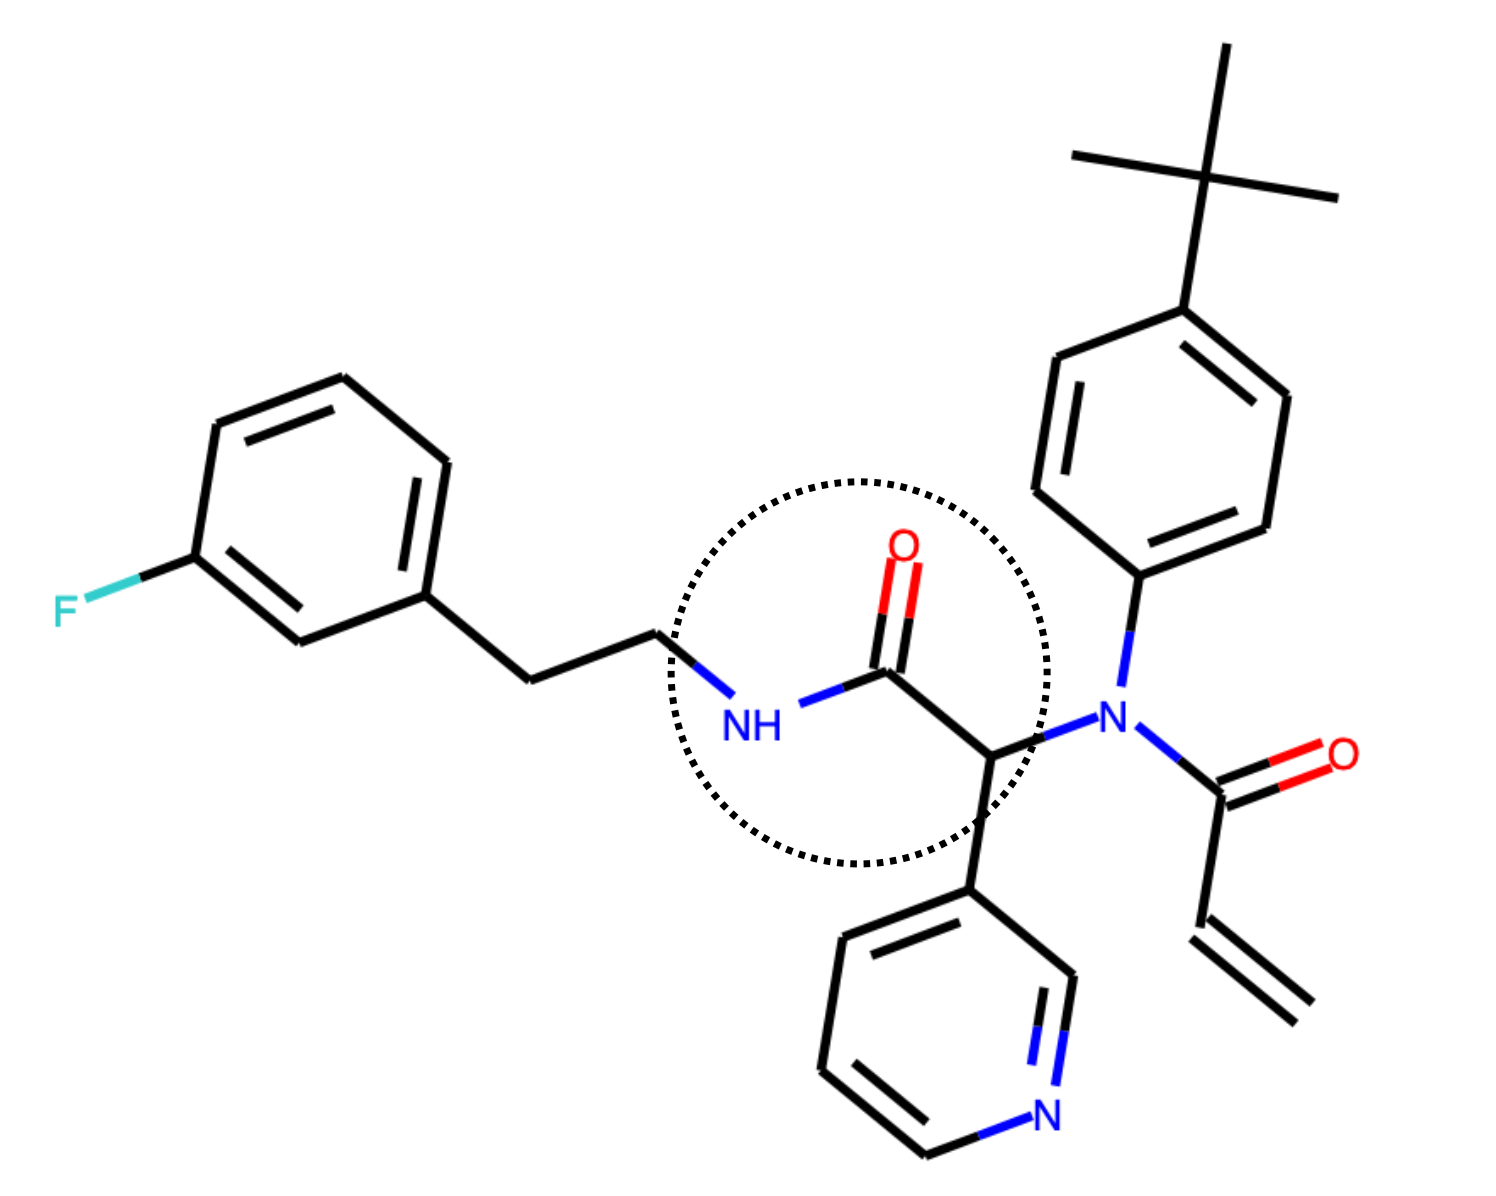
\includegraphics[width=0.5\textwidth]{Chapter3/Figs/example_mol.png}
% \caption{\label{fig:example} An example of a potent molecule (IC50 = $2.96\mu$M) where the amide/urea motif is highlighted with the dashed circle.}
% \end{figure}

% For the non-covalents, the procedure was therefore to slice along all amide and urea bonds as well as the slicing the substituents from secondary amines. All possible secondary amines were then enumerated by combining all substituents with all primary amines, and all primary/secondary amines were then combined with all substituents to obtain a library of amides and ureas. This resulted in a library of size $\sim$870k. For the acrylamides the procedure is more straightforward, simply being an enumeration of all possible Ugi reaction components (carboxylic acids, primary amines, ketone/aldehydes, and isocyanides) in the dataset. The primary amines derived from the non-covalents were also included in the enumeration process, resulting in a library of size $\sim$11k. 


Figure \ref{fig:roc_plot} shows that our binary ranking model achieves an AUC of 0.88 (95\% CI: [0.83,0.96]) in ranking ligands within the test set, and AUC for 0.94 (95\% CI: [0.91,0.98]) where we compare a ligand in the training set against another ligand in the test set; the latter is more relevant as our goal is finding ligands more active than the best incumbent. The 95\% confidence interval is computed using bootstrapping. We also compare our model against OpenEye’s FRED hybrid docking mode as implemented in the ``Classic OEDocking'' floe, a physics-based docking algorithm, on the Orion online platform, which achieves AUC of 0.72; 95\% CI: [0.722,0.723] (see ESI for implementation details). Note that docking does not require ligand bioactivity as training data, thus is not a directly comparison to machine learning. In the Supplementary Material, we discuss that our model ranks ligands better than a model that directly learns $\mathrm{IC}_{50}$ (AUC = 0.86; 95\% CI: [0.71,0.95]). 

Beyond train-test split, model performance can be evaluated from a time-split. Five months have elapsed from the time we deployed our model to select compounds to writing up the manuscript. During that time, the COVID Moonshot Consortium (a team of expert medicinal chemists) has independently designed, synthesised and tested 356 compounds \cite{moonshot2020covid}, out of which 15\% were better than the top 2 compounds (having $\mathrm{IC}_{50}$ comparable within error) in our dataset. Table \ref{table:time_split} shows that our model has an enrichment factor of $\sim$2, i.e. if we rescore the 356 compounds synthesized by the medicinal chemistry team using our model, and pick the top 1\%-10\% percentile, the proportion of molecules that would be better than the top 2 compounds would be $\sim$2x higher than human selection. 

%From a set of binary ranking, we can accurately rank-order the active ligands (Figure XXXb), with a higher rank correlation than using the quantitative activity data alone. We use the average probability of a ligand being ranked higher than ligands in the training set as a proxy for overall rank.

\begin{figure}
\centering
    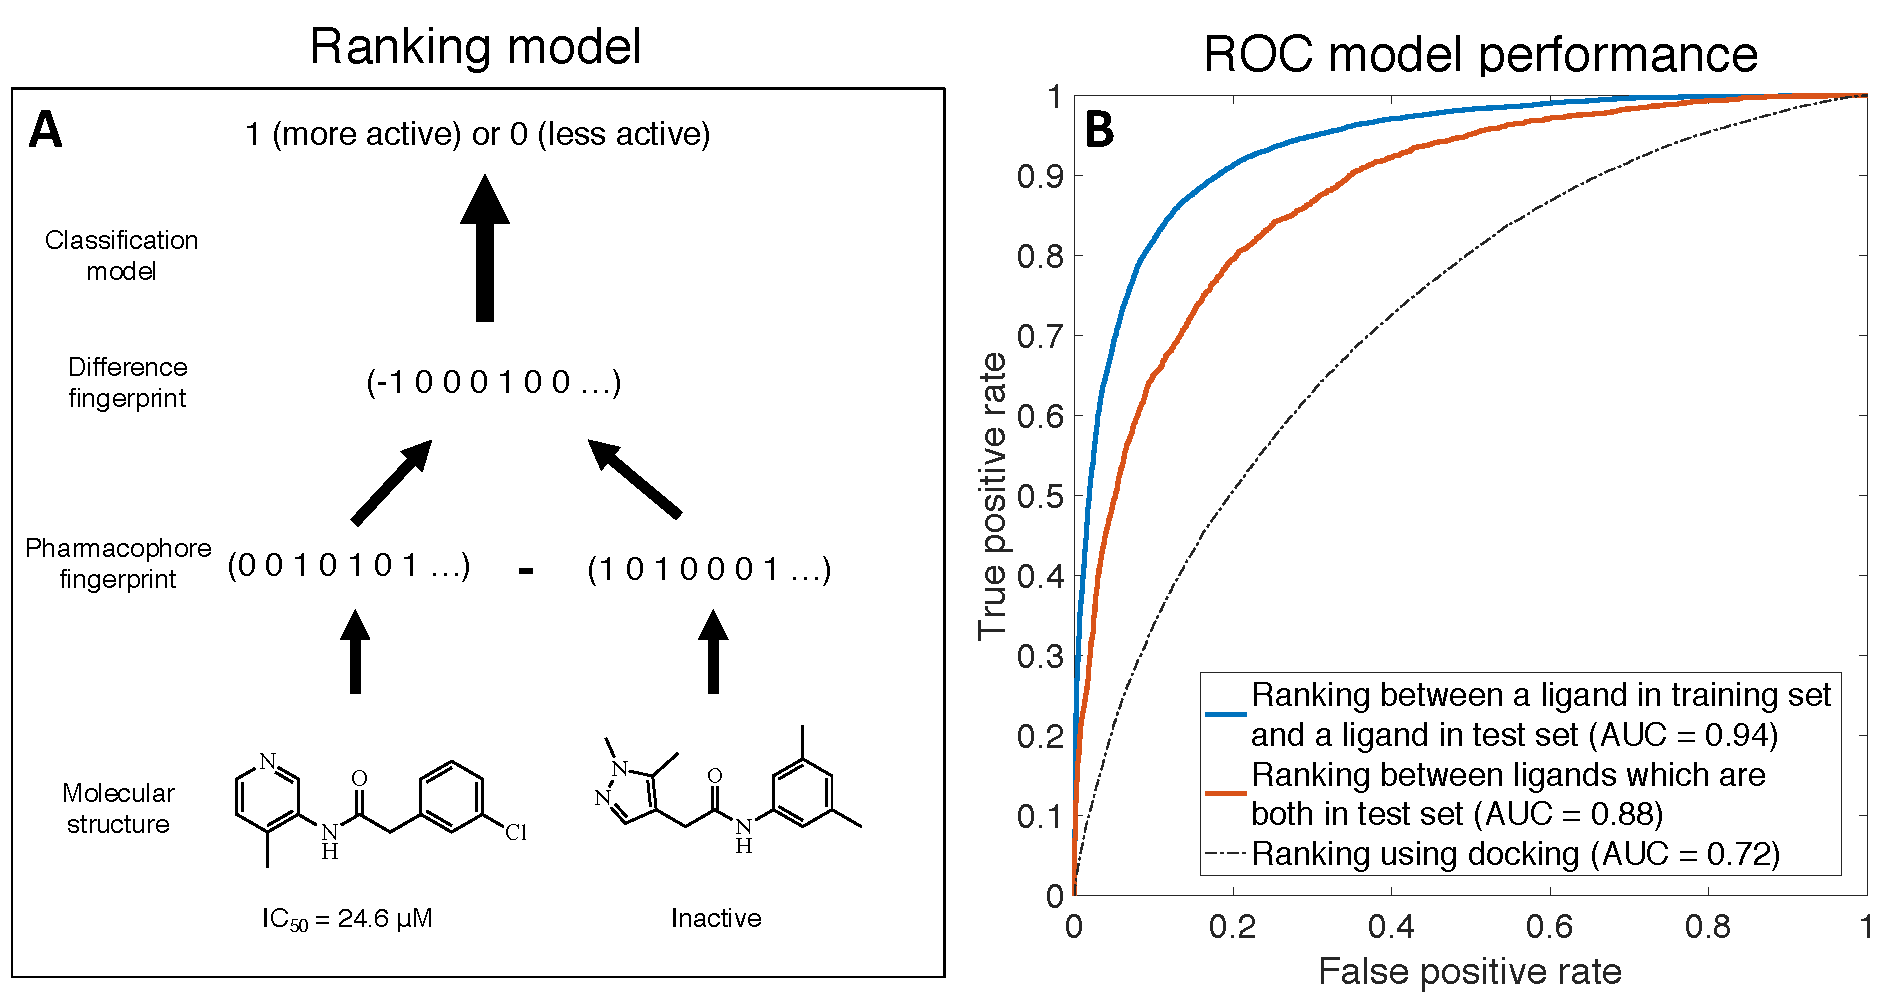
\includegraphics[scale=0.28]{Chapters/Ranking/Figs/ranking-model.pdf}
    \caption{Relative ranking of ligands can be predicted by our learning-to-rank machine learning model. (A) A schematic of the model setup. A classifier takes the difference in pharmacophore fingerprint between two molecules and predicts where one molecule is more or less active than the other. (B) The Receiver Operating Characteristic curve of classifying whether a molecule is more/less active than the other. AUC 95\% CI reported in main text.}
    \label{fig:roc_plot}
\end{figure}

\begin{table}
\centering
\begin{tabular}{|l|l|l|l|}
\hline
\textbf{Percentile}        & 1\% & 2.5\% & 10\% \\ \hline
\textbf{Enrichment Factor} & 1.7 & 2.3   & 1.7  \\ \hline
\end{tabular}
\caption{Enrichment factor for the time-split dataset, where we consider model performance on data arriving after the model has been deployed to generate compounds for synthesis and testing. }
\label{table:time_split}
\end{table}

\begin{figure}
\centering
         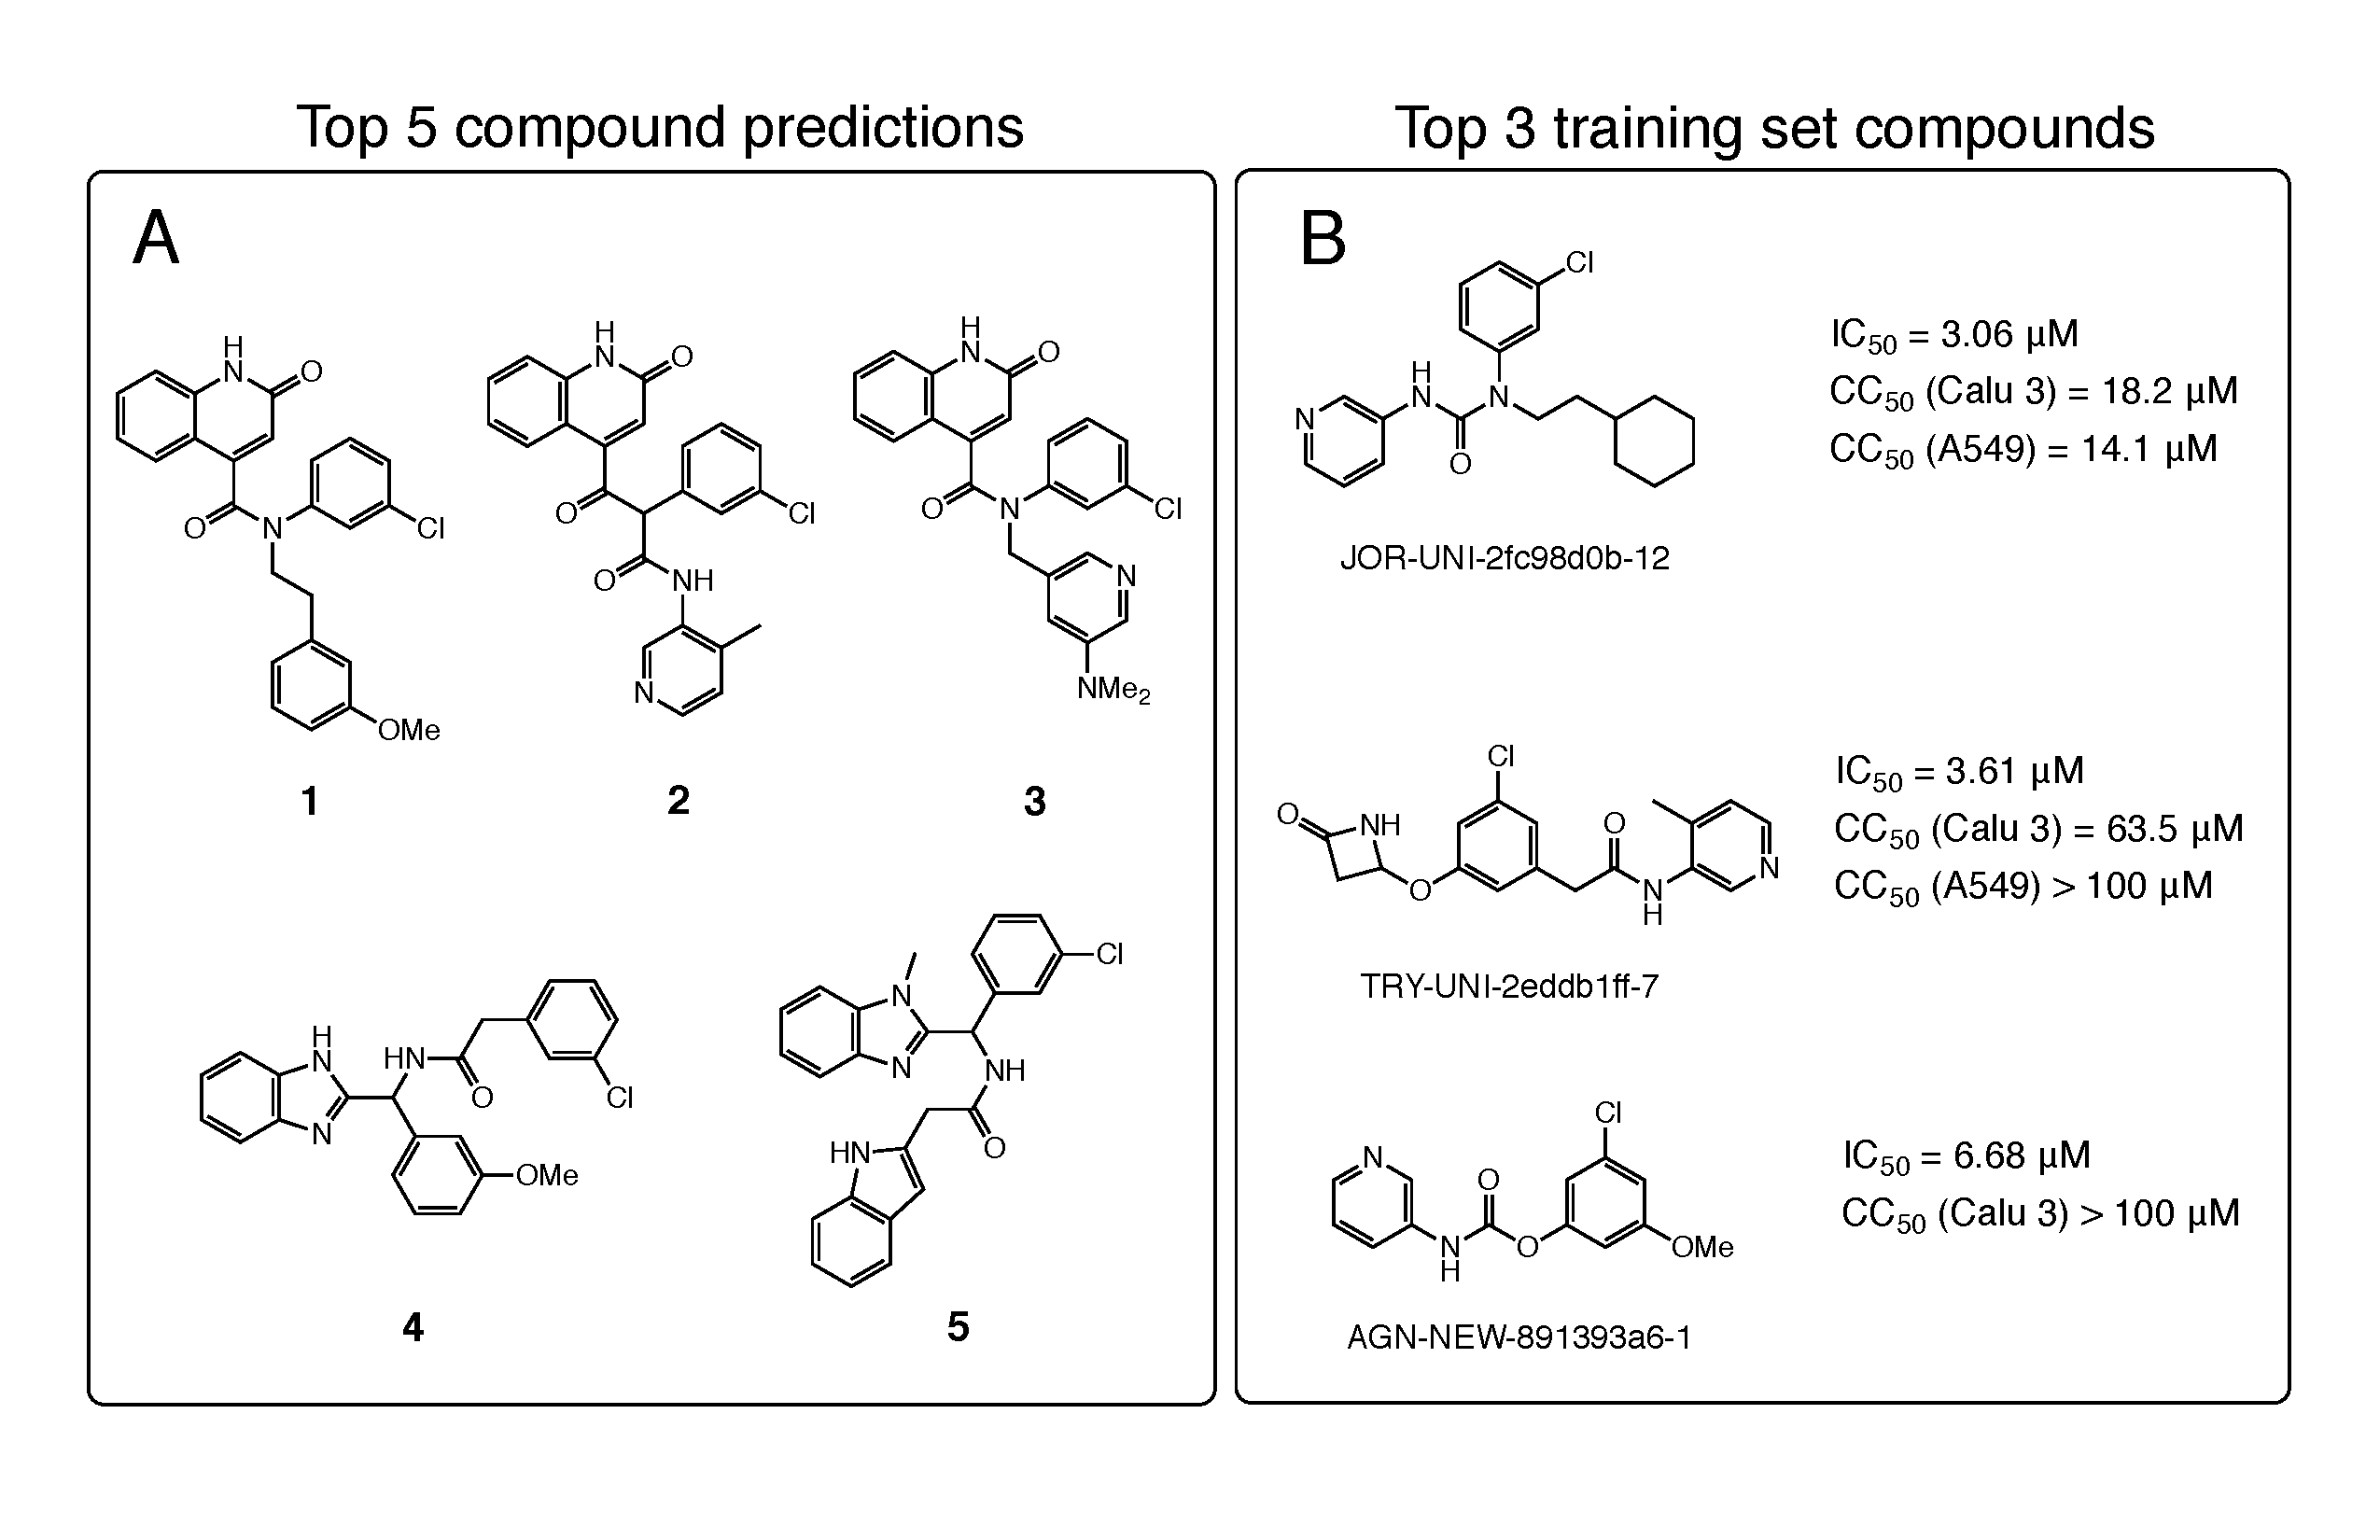
\includegraphics[width=0.45\textwidth]{Chapters/Ranking/Figs/fig2.pdf}
    \caption{Our synthesis-driven design model prioritises molecular scaffold that are not in the top hits. (A) The 5 compounds selected by our methodology for synthesis and testing. (B) The top 3 compounds from the training set, with potency and cytotoxicity measurements. }
    \label{fig:compounds}
\end{figure}

%describe our generative model + schematic 

%TODO - discuss this approach more in depth (examples in literature)

Having demonstrated the accuracy of our ranking model, we now turn to chemical space exploration. We first consider a set of chemically reasonable perturbations (e.g. amide to retroamide, amide to urea), which is applied to the whole set of active molecules. We then fragment along synthetically accessible bonds (e.g. amides and aromatic C-C and C-N), and reconnect the synthons to generate an exhaustive library. The resulting library of 8.8 million generated molecules is scored using our ranking model by the probability of having a higher potency compared to the most potent molecule in the dataset.  % We use a simple scheme based on breaking along synthetically accessible bonds. 


\begin{figure}
\centering
         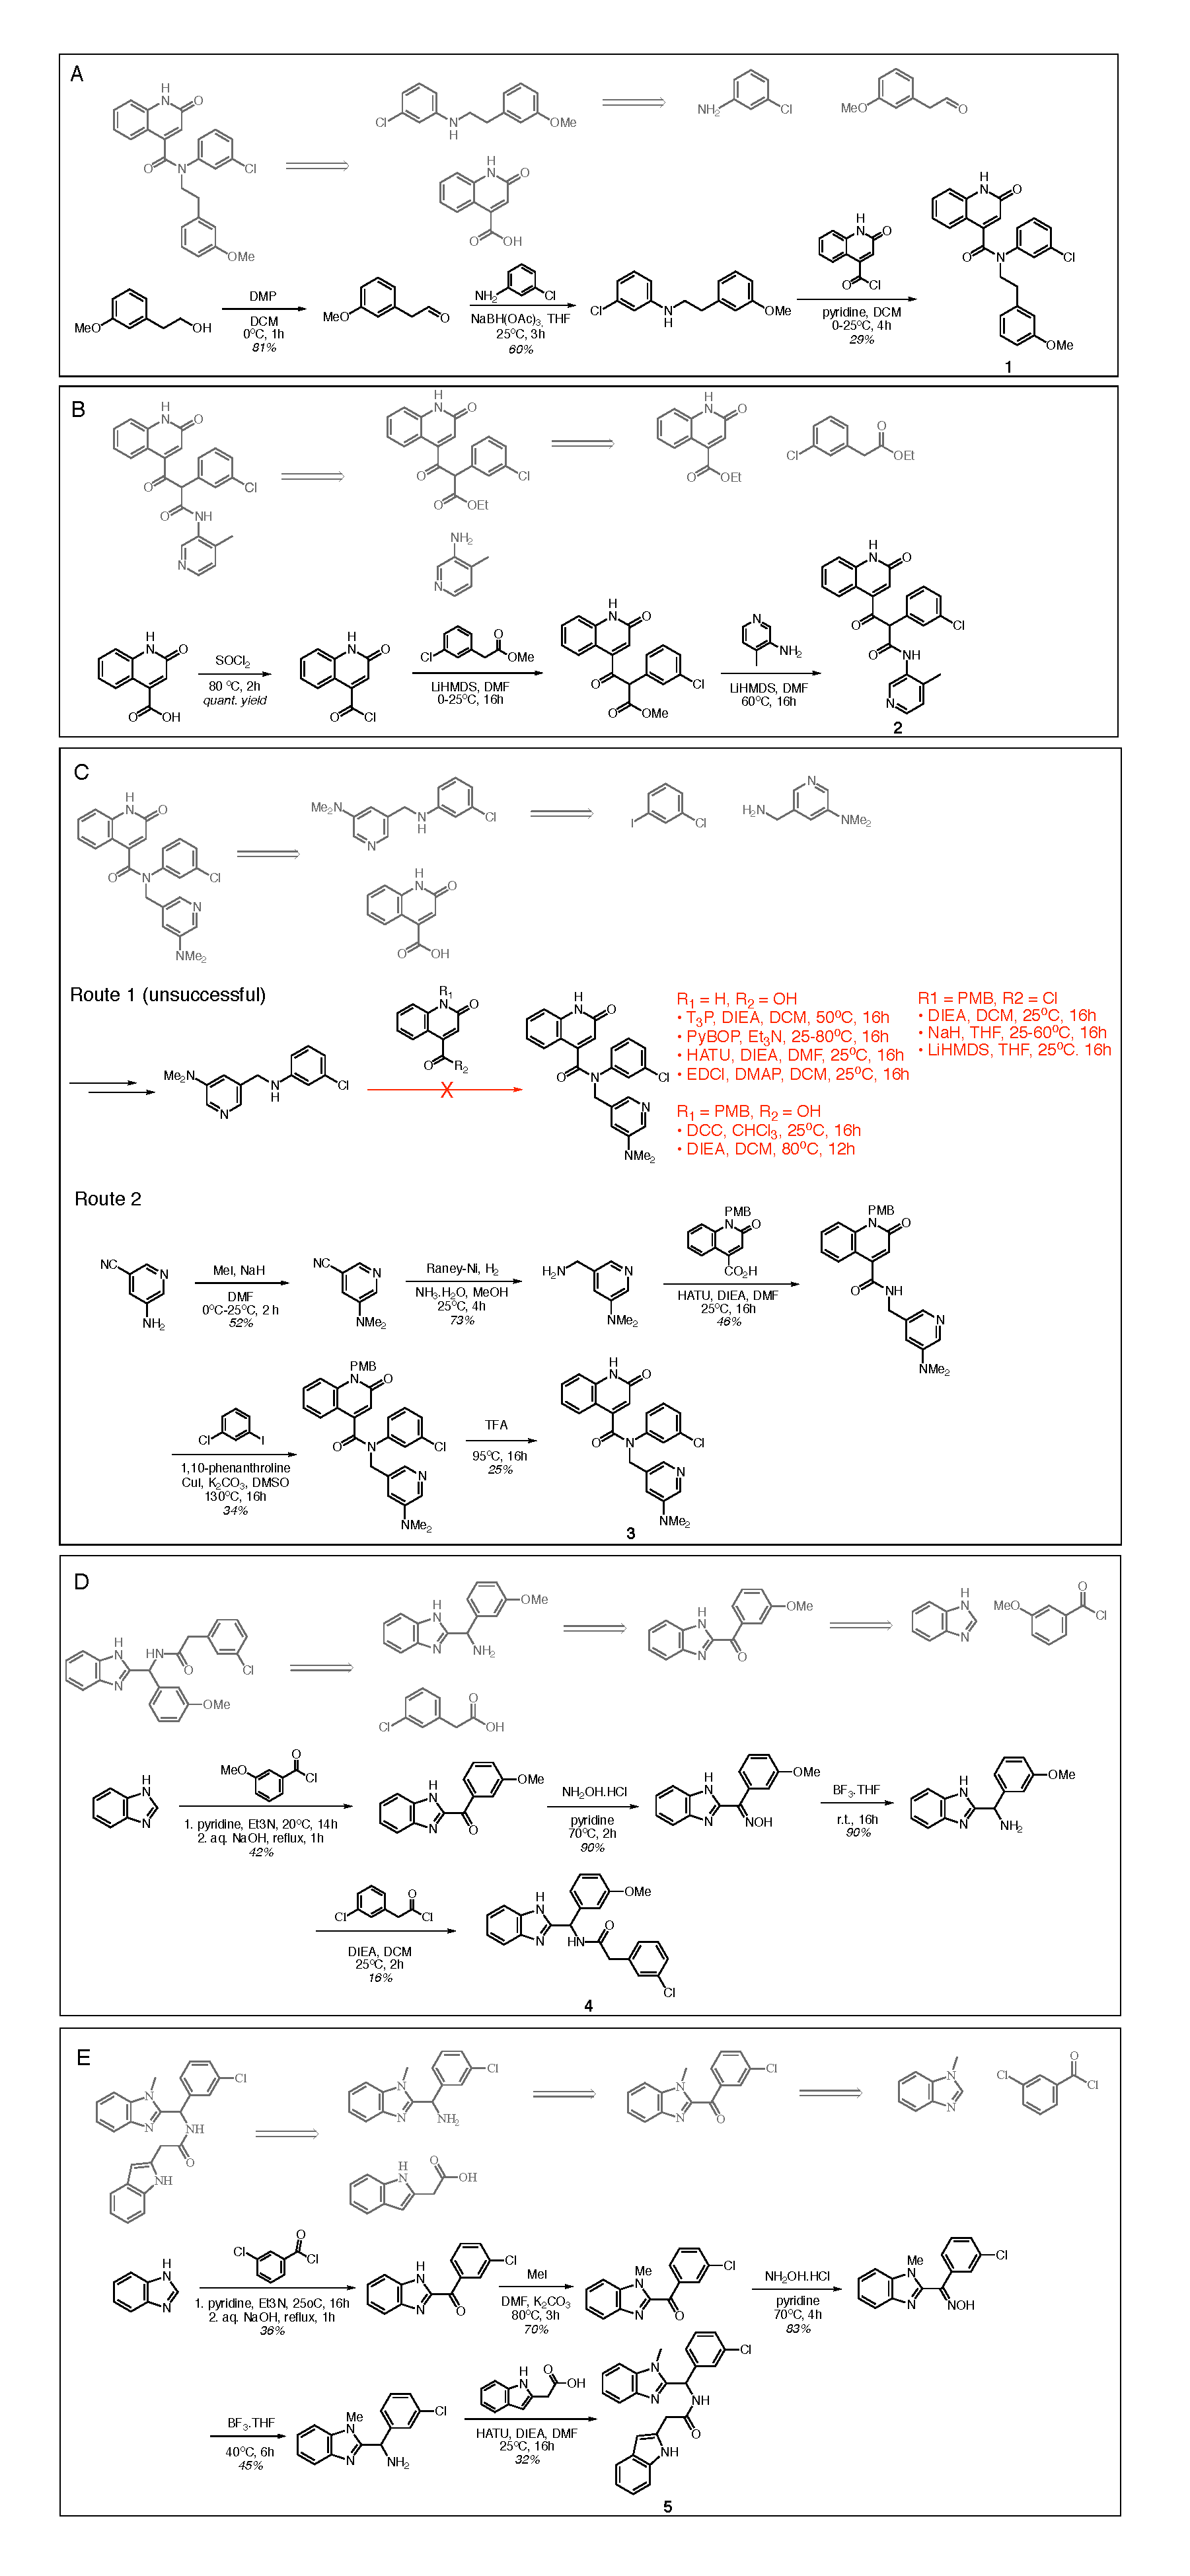
\includegraphics[width=0.5\textwidth]{Chapters/Ranking/Figs/aaron_schemes.pdf}
    \caption{Model generated synthetic schemes that are experimentally validated. Schemes (A)-(E) show the synthesis schemes generated by our model (grey) and experimental schemes for Compounds $\mathbf{1}$-$\mathbf{5}$. The ESI contains experimental procedures provided by our contract research organisation.}
    \label{fig:synthesis_schemes}
\end{figure}

Although virtual ``reactions'' were used to generate new molecules, the synthons are not necessarily off-the-shelf nor the reactions optimal. As such, we use a retrosynthesis predictor to triage based on synthetic accessibility. We fed top hits into Manifold, our platform for synthesis route prediction (\url{https://postera.ai/manifold}). Manifold searches for synthetic routes starting from purchasable molecules. The underlying technology is based on Molecular Transformer, a machine learning model for reaction prediction using sequence-to-sequence translation \citep{yang2019molecular,schwaller2019molecular}. The top 5 molecules with predicted routes <4 steps were synthesised and tested (Figure \ref{fig:compounds}A). For comparison, the most potent molecules from the training set are shown in Figure \ref{fig:compounds}B; $\mathbf{1}-\mathbf{5}$ have Tanimoto similarity <0.48 (1024-bit ECFP6) to every molecule in the training set. 

%TODO - remove unnecessary detail about retrosynthesis
Figure \ref{fig:synthesis_schemes} shows that for Compounds $\mathbf{1}$, $\mathbf{2}$, $\mathbf{4}$ and $\mathbf{5}$ our retrosynthesis algorithm generates successful routes, thus provides a reasonable estimate of synthetic complexity. The syntheses were carried out at the Wuxi AppTec and compounds were assayed as received. Minor variations in building blocks were employed depending on what was readily available. We note that our algorithm failed to estimate the synthetic complexity of Compound $\mathbf{3}$. The final amide formation step was unexpectedly challenging, and no desired product was seen despite significant efforts in condition screening. Compound $\mathbf{3}$ was furnished via an alternative strategy, employing an Ullmann coupling to arylate the amide, which was not predicted by our approach. 

%result + discussion 
Compounds $\mathbf{1}$-$\mathbf{5}$ were tested for Mpro activity using a fluorescence assay. Figure \ref{fig:data} shows that Compounds $\mathbf{1}$-$\mathbf{3}$ have $\mathrm{IC}_{50}$ within assay dynamic range ($<100 \mu M$), and Compound $\mathbf{1}$ has $\mathrm{IC}_{50} = 4.1 \mu M$. Compound $\mathbf{1}$ is further assayed in live virus assays, with the less pathogenic OC43 coronavirus, showing $\mathrm{EC}_{50} = 13 \mu M$ and is not cytotoxic ($\mathrm{CC}_{50}>100 \mu M$ against A549 cell line; $CC_{50}$ is the concentration required  to cause 50\% cell death). We employ OC43 as a rapid surrogate assay for SARS-CoV-2 as the former can be done in a BSL-2 rather than BSL-3 lab.  Interestingly, the top non-cytotoxic hit of the training set (TRY-UNI-2eddb1ff-7) does not show OC43 activity, showcasing the utility of using generative models to suggest new scaffolds with complementary physicochemical properties. 

\begin{figure}
\centering
         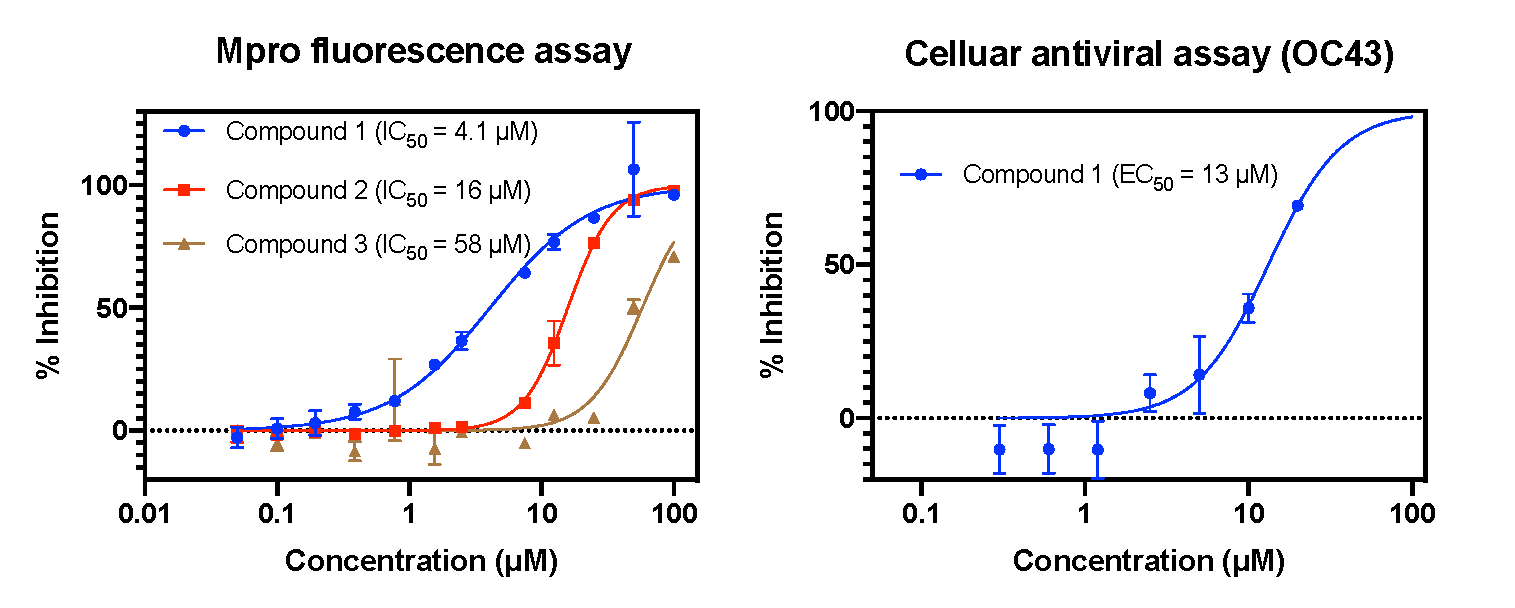
\includegraphics[scale=0.36]{Chapters/Ranking/Figs/data_curve.pdf}
    \caption{Three compounds generated using our synthesis-directed model exhibit Mpro activity. Our most active compound has measurable antiviral activity against the OC43 coronavirus and no measurable cytotoxic effect ($\mathrm{CC}_{50} (A549)>100 \mu M$). 95\% CI: IC50 (Mpro) -- Compound 1 [3.42,4.86] $\mu$M, Compound 2 [15.1,16.5] $\mu$M, Compound 3 [48.8,69.4] $\mu$M; EC50 (OC43) -- Compound 1 [10.1, 18.4] $\mu$M. See ESI for assay details.}
    \label{fig:data}
\end{figure}

\section{Discussion} \label{sec:discussion}

In summary, we demonstrated the utility of a \emph{de novo} design model, guided by estimation of synthetic complexity, for generating ideas in hit expansion. At the time of writing, the quinolone series is undergoing optimisation by the COVID Moonshot initiative (\url{https://postera.ai/covid}). Data for Compound $\mathbf{1}$-$\mathbf{5}$ is registered as the $\texttt{ALP-POS-ddb41b15}$ series on the Moonshot platform. 

\section{Fluorescence MPro inhibition assay}

Compounds were seeded into assay-ready plates (Greiner 384 low volume 784900) using an Echo 555 acoustic dispenser, and DMSO was back-filled for a uniform concentration in assay plates (maximum 1\%). Screening assays were performed in duplicate at 20 $\mu$M and 50 $\mu$M. Hits of greater than 50 \% inhibition at 50 $\mu$M were confirmed by dose response assays. Reagents for Mpro assay reagents were dispensed into the assay plate in 10 µl volumes for a final volume of 20 $\mu$L. 
Final reaction concentrations were 20 mM HEPES pH 7.3, 1 mM TCEP, 50 mM NaCl, 0.01\% Tween-20, 10\% glycerol, 5nM Mpro, 375nM fluorogenic peptide substrate ([5-FAM]-AVLQSGFR-[Lys(Dabcyl)]-K-amide). 
Mpro was pre-incubated for 15 minutes at room temperature with compound before addition of substrate. Protease reaction was measured continuously in a BMG Pherastar FS with a 480/520 ex/em filter set. Data analysis was performed with Collaborative Drug Discovery (CDD).

\section{OC43 antiviral assay}

A549 expressing H2B-mRuby were seeded in 384 well plates (4,000 cells per well) in DMEM+2\% FCS in a total volume of 30ul. One day later, 20ul of OC43 were added to the wells for a final MOI of 0.3. one hour after viral addition, the drug (or DMSO as control) was added to the cells. Drugs were added at a volume of 50nl, in a final dose range of 0.3-20mM. Cells were incubated at 33C, 5\% CO2 for 2 days, fixed with paraformaldehyde and stained for the presence of the viral nucleoprotein. Images were captured and quantified using the Incucyte machine and software. 3 biological repeated were performed.

\section{Compound Synthesis}

Compounds 1-5 were sourced from Wuxi AppTec and used as received. Synthesis routes reported by Wuxi AppTec is appended in the ESI. 


\section{Learning-to-rank} 

Our learning-to-rank methods converts ranking into binary classification of whether a compound is more/less active than another compound. This allows us to assimilate both coarse (active/inactive) and fine (quantitative potency measurements) into a single model. All inactive compounds are less active than active compounds, and compounds with potency measurements are ranked by their potency.  

To represent a molecule, we concatenate 3 fingerprint representations implemented in \texttt{rdkit}, all 512 bits each into one 1536 representation: Morgan, Atom, TopologicalTorsion. The fingerprint is projected onto 20 dimensions using Principal Component Analysis. The input to the model is the difference in fingerprint between two molecules, $f_A - f_B$, and the output is the whether the molecule $A$ is more or less potent that molecule $B$ -- i.e. a classification problem. Note that this creates a balanced classification dataset.  

The classifier we employ is the FastAI tabular model, a general machine learning package for processing classification problems. 

Source code of our method can be found in: \url{https://github.com/wjm41/mpro-rank-gen/tree/main/rank_model}.  

\section{Compound generation} 
To generate new compounds, we: (a)introduce linker and chemotype swaps, e.g. amide to retroamide, amide to urea, swapping N-aryl groups; (b) fragment compounds along synthetically accessible bonds into building blocks, e.g. amide to carboxylic acid and amine; (c) reconnect the fragments to form a library of virtual compounds. These operations are defined using SMARTS rules. 

The virtual library of compounds is then scored against the top 4 compound in the training set using the learning-to-rank framework. Compounds predicted to have higher activity is then fed into our synthetic route predictor \cite{schwaller2019molecular,yang2019molecular}. 5 molecules with $<$4 predicted steps were synthesised and assayed. 


\section{Docking workflow} 

As a baseline comparison, we docked the training and test sets of our machine learning model against x2908 structure reported by Diamond XChem \cite{douangamath2020crystallographic}.  We use the ``Classic OEDocking'' floe v0.7.2 as implemented in the Orion 2020.3.1 Academic Stack (OpenEye Scientific). Omega was used to enumerate conformations (and expand stereochemistry) with up to 500 conformations. \texttt{FRED} was used for docking in \texttt{HYBRID} mode using the x2908 bound ligand. 


\section{Retrospective performance analysis} 

We compare the performance of our model in predicting the pairwise ranking of compounds against the baseline model of simply training a regression model on bioactivities. As a baseline model, we trained a random forest model with the package \texttt{scikit-learn} \cite{scikit-learn}, \texttt{RandomForestRegressor} function, with default hyperparameters. Likewise, for the learning-to-rank model we take the FastAI tabular model with default hyperparameters, as discussed in the main text. 

    
\begin{table}[]
\centering
\begin{tabular}{|l|l|l|}
\hline
\textbf{Dataset} & \textbf{RF Baseline AUC} & \textbf{Model AUC}  \\ \hline
LCK              & 0.94              & 0.91          \\ \hline
opioid           & 0.92                & \textbf{0.94} \\ \hline
Cannabinoid      & 0.97               & 0.87          \\ \hline
Estrogen         & 0.96               & \textbf{0.98} \\ \hline
B-raf            & 0.95              & \textbf{0.96} \\ \hline
Ephrin           & 0.83               & \textbf{0.85} \\ \hline
Glycogen         & 0.89             & 0.88         \\ \hline
Vanilloid        & 0.93              & 0.90          \\ \hline
JAK2             & 0.97              & \textbf{0.98} \\ \hline
Dopamine         & 0.97               & \textbf{0.98} \\ \hline
ABL1             & 0.81               & \textbf{0.84} \\ \hline
A2a              & 0.58              & \textbf{0.91} \\ \hline
Coagulation      & 0.82                & \textbf{0.85}  \\ \hline
Glucocorticoid   & 0.96             & \textbf{0.98} \\ \hline
Dihydrofolate    & 0.90               & 0.86          \\ \hline
Carbonic         & 0.97              & \textbf{0.996} \\ \hline
Aurora-A         & 0.89               & \textbf{0.93} \\ \hline
\end{tabular}
\caption{Comparing learning-to-rank with direct potency prediction in prioritising compounds.}
\label{table1}
\end{table}
